%%%%%%%%%%%%%%%%%%%%%%%%%%%%%%%%%%%%%%%%%%%%%%%%%%%%%%%%%%%%%%%%%%%%%%%%%%%
%% This file is part of the book
%%
%% Algorithmic Graph Theory
%% http://code.google.com/p/graph-theory-algorithms-book/
%%
%% Copyright (C) 2009, 2010, 2011 Minh Van Nguyen <nguyenminh2@gmail.com>
%%
%% See the file COPYING for copying conditions.
%%%%%%%%%%%%%%%%%%%%%%%%%%%%%%%%%%%%%%%%%%%%%%%%%%%%%%%%%%%%%%%%%%%%%%%%%%%

\documentclass{article}

\usepackage{tikz}
\usetikzlibrary{external}
\usetikzlibrary{matrix}
\tikzexternalize{Euler-polygon-division-hexagon}

\begin{document}

\begin{figure}
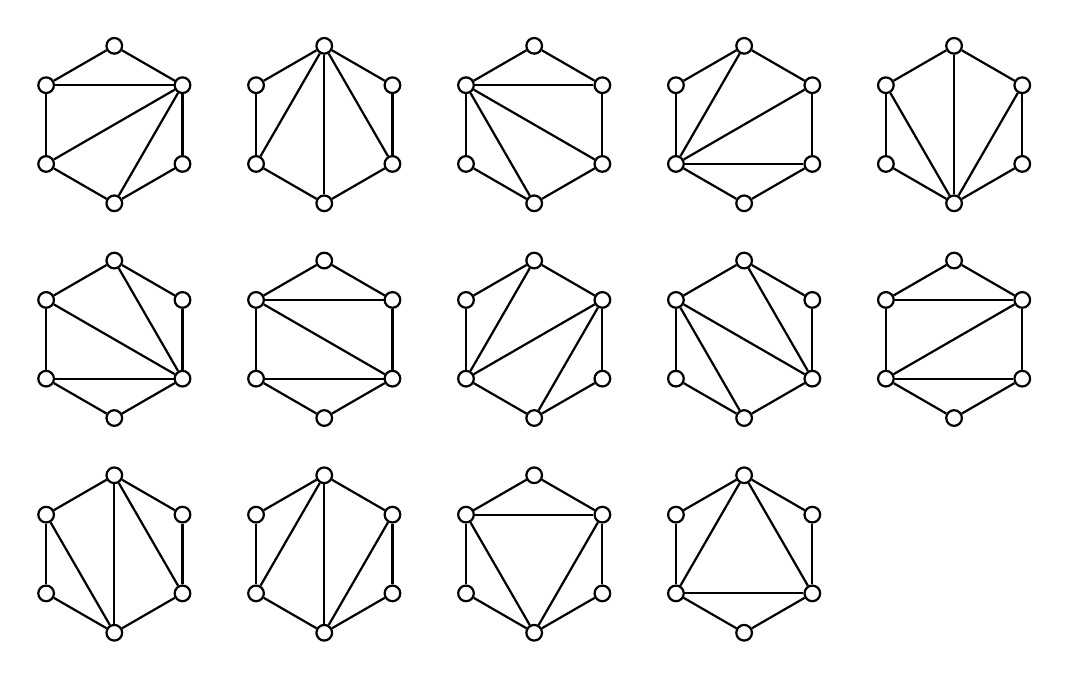
\begin{tikzpicture}
[linedecorate/.style={-,thick},%
  nodedecorate/.style={shape=circle,inner sep=2pt,draw,thick}]
%%
%% Macros
%% Hexagon
\def\hexagon{%
  %% nodes or vertices
  \foreach \nodename/\x/\y in {
    A/0.8660/0.5, B/0/1, C/-0.8660/0.5, D/-0.8660/-0.5, E/0/-1, F/0.8660/-0.5}
  {
    \node (\nodename) at (\x,\y) [nodedecorate] {};
  }
  %% edges or lines
  \path
  \foreach \startnode/\endnode in {A/B, B/C, C/D, D/E, E/F, F/A} {
    (\startnode) edge[linedecorate] node {} (\endnode)
  };
}
%% Polygon diagonals
\newcommand{\slice}[1]{%
  \hexagon
  \path
  \foreach \startnode/\endnode in {#1} {
    (\startnode) edge[linedecorate] node {} (\endnode)
  };
}
%%
%% Draw the sliced hexagons
\matrix[column sep=0.7cm,row sep=0.5cm]{
  \slice{A/C,A/D,A/E} &
  \slice{B/D,B/E,B/F} &
  \slice{C/A,C/E,C/F} &
  \slice{D/B,D/F,D/A} &
  \slice{E/A,E/B,E/C} \\
  \slice{F/B,F/C,F/D} &
  \slice{A/C,C/F,F/D} &
  \slice{B/D,D/A,A/E} &
  \slice{B/F,F/C,C/E} &
  \slice{C/A,A/D,D/F} \\
  \slice{C/E,E/B,B/F} &
  \slice{D/B,B/E,E/A} &
  \slice{A/C,C/E,E/A} &
  \slice{B/D,D/F,F/B} \\
};
\end{tikzpicture}
\end{figure}

\end{document}
